\documentclass{standalone}
\usepackage[utf8]{inputenc}
\usepackage{amsmath}
\usepackage{amssymb}

\usepackage{tikz}
\usetikzlibrary{shapes.geometric, arrows}

\tikzstyle{startstop} = [rectangle, rounded corners, minimum width=3cm, minimum height=1cm,text centered, draw=black, fill=red!30]
\tikzstyle{io} = [trapezium, trapezium left angle=70, trapezium right angle=110, minimum width=3cm, minimum height=1cm, text centered, draw=black, fill=blue!30]
\tikzstyle{process} = [rectangle, minimum width=3cm, minimum height=1cm, text centered, draw=black, fill=orange!30]
\tikzstyle{decision} = [diamond, minimum width=3cm, minimum height=1cm, text centered, draw=black, fill=green!30]
\tikzstyle{arrow} = [thick,->,>=stealth]
\tikzstyle{fdot} = [circle, minimum width=8pt, fill]
\tikzstyle{line} = [thick,>=stealth]

\begin{document}

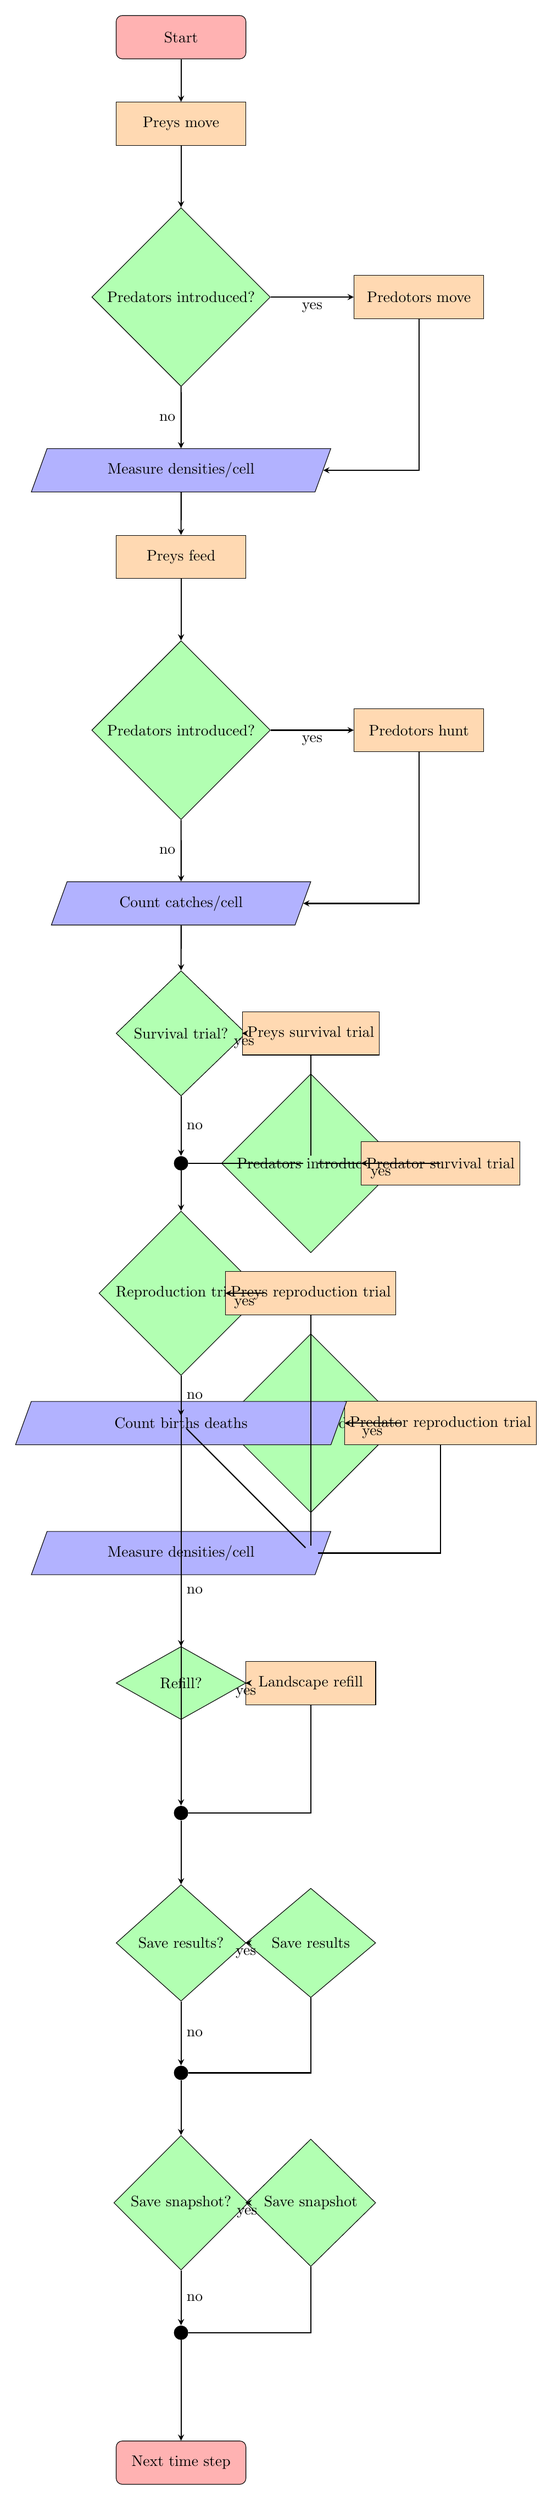
\begin{tikzpicture}[scale=0.5, node distance=3cm]

\node (start) [startstop] {Start};
\node (pro1) [process, below of=start, yshift=1cm] {Preys move};
\node (dec1) [decision, below of=pro1, yshift=-1cm] {Predators introduced?};
\node (pro2) [process,  right of=dec1, xshift=2.5cm] {Predotors move};
\node (io1) [io, below of=dec1, yshift=-1cm] {Measure densities/cell};
\node (pro3) [process, below of=io1, yshift=1cm] {Preys feed};
\node (dec2) [decision, below of=pro3, yshift=-1cm] {Predators introduced?};
\node (pro4) [process,  right of=dec2, xshift=2.5cm] {Predotors hunt};
\node (io2) [io, below of=dec2, yshift=-1cm] {Count catches/cell};
\node (dec3) [decision, below of=io2] {Survival trial?};
\node (pro5) [process,  right of=dec3] {Preys survival trial};
\node (fdot1) [fdot, below of=pro5] {};
\node (dec4) [decision, below of=pro5] {Predators introduced?};
\node (pro6) [process,  right of=dec4] {Predator survival trial};
\node (fdot2) [fdot, below of=dec3] {};
\node (dec5) [decision, below of=fdot2] {Reproduction trial?};
\node (pro7) [process,  right of=dec5] {Preys reproduction trial};
\node (dec6) [decision, below of=pro7] {Predators introduced?};
\node (fdot3) [fdot, below of=dec6] {};
\node (pro8) [process,  right of=dec6] {Predator reproduction trial};
\node (fdot4) [fdot, below of=dec5] {};
\node (io3) [io, below of=dec5] {Count births deaths};
\node (io4) [io, below of=io3] {Measure densities/cell};
\node (dec7) [decision, below of=io4] {Refill?};
\node (pro9) [process,  right of=dec7] {Landscape refill};
\node (fdot5) [fdot, below of=dec7] {};
\node (dec8) [decision, below of=fdot5] {Save results?};
\node (pro10) [decision, right of=dec8] {Save results};
\node (fdot6) [fdot, below of=dec8] {};
\node (dec9) [decision, below of=fdot6] {Save snapshot?};
\node (pro11) [decision, right of=dec9] {Save snapshot};
\node (fdot7) [fdot, below of=dec9] {};
\node (stop) [startstop, below of=fdot7] {Next time step};

\draw [arrow] (start) -- (pro1);
\draw [arrow] (pro1) -- (dec1);
\draw [arrow] (dec1) -- node[anchor=north] {yes} (pro2);
\draw [arrow] (dec1) -- node[anchor=east] {no} (io1);
\draw [arrow] (pro2) |- (io1);
\draw [arrow] (io1) -- (pro3);
\draw [arrow] (pro3) -- (dec2);
\draw [arrow] (dec2) -- node[anchor=north] {yes} (pro4);
\draw [arrow] (dec2) -- node[anchor=east] {no} (io2);
\draw [arrow] (pro4) |- (io2);
\draw [arrow] (io2) -- (dec3);
\draw [arrow] (dec3) -- node[anchor=north] {yes} (pro5);
\draw [arrow] (dec3) -- node[anchor=west] {no} (fdot2);
\draw [line] (pro5) -- (fdot1);
\draw [arrow] (dec4) -- node[anchor=north] {yes} (pro6);
\draw [line] (pro6) |- (fdot1);
\draw [line] (fdot1) -- (fdot2);
\draw [arrow] (fdot2) -- (dec5);
\draw [arrow] (dec5) -- node[anchor=north] {yes} (pro7);
\draw [arrow] (dec5) -- node[anchor=west] {no} (fdot4);
\draw [line] (pro7) -- (fdot3);
\draw [arrow] (dec6) -- node[anchor=north] {yes} (pro8);
\draw [line] (pro8) |- (fdot3);
\draw [line] (fdot3) -- (fdot4);
\draw [arrow] (fdot4) -- (dec7);
\draw [arrow] (dec7) -- node[anchor=north] {yes} (pro9);
\draw [arrow] (dec5) -- node[anchor=west] {no} (fdot5);
\draw [line] (pro9) |- (fdot5);
\draw [arrow] (fdot5) -- (dec8);
\draw [arrow] (dec8) -- node[anchor=north] {yes} (pro10);
\draw [arrow] (dec8) -- node[anchor=west] {no} (fdot6);
\draw [line] (pro10) |- (fdot6);
\draw [arrow] (fdot6) -- (dec9);
\draw [arrow] (dec9) -- node[anchor=north] {yes} (pro11);
\draw [arrow] (dec9) -- node[anchor=west] {no} (fdot7);
\draw [line] (pro11) |- (fdot7);
\draw [arrow] (fdot7) -- (stop);

\end{tikzpicture}

\end{document}